%%%%%%%%%%%%%%%%%%
% BEGIN PREAMBLE %
%%%%%%%%%%%%%%%%%%

\documentclass[12pt,a4paper]{amsart}

\pagestyle{plain}
\addtolength{\oddsidemargin}{-0.8in}
\addtolength{\evensidemargin}{-0.8in}
\addtolength{\textwidth}{1.6in}

\addtolength{\topmargin}{-1in}
\addtolength{\textheight}{1in}

\usepackage{amssymb,amscd,amsmath,amsthm,url,microtype,graphicx,braket,xcolor,csquotes,fontawesome,MnSymbol,chessfss}

\usepackage{tikz}

\usepackage[a6paper,top=10mm,bottom=15mm,left=10mm,right=10mm]{geometry}


\newtheorem*{Theorem}                    {Theorem}
\newtheorem {Proposition}       {Proposition}
\newtheorem {Lemma}             {Lemma}
\newtheorem {Corollary}   {Corollary}
\newtheorem*{Claim}       {Claim}
\newtheorem*{Question}   {Question}
\newtheorem*{Exercise}   {Exercise}

\theoremstyle{definition}
\newtheorem*  {Definition} {Definition}
\newtheorem  {Joke} {Joke}
\newtheorem{Example}{Example}

\theoremstyle{remark}
\newtheorem*{Remark}	{Remark}



\newcommand{\mute}[1] {}

\newcommand{\mc}[1]{\mathcal{#1}}
\newcommand{\mf}[1]{\mathfrak{#1}}
\newcommand{\mbb}[1]{\mathbb{#1}}
\newcommand{\cal}[1]{\mathcal{#1}}

\def \N{\mathbb{N}}
\def \Z{\mathbb{Z}}
\def \R{\mathbb{R}}
\def \C{\mathbb{C}}
\def \Q{\mathbb{Q}}
\def \H{\mathbb{H}}

\def \vphi{\varphi}
\def \eps{\varepsilon}
\def \ssm{\smallsetminus}
\def \del{\partial}

%%%%%%%%%%%%%%%%
% END PREAMBLE %
%%%%%%%%%%%%%%%%

% This begins the document
%\pagenumbering{gobble}
\graphicspath{{./Images/}}
\begin{document}
\begin{center}
  \begin{figure}[ht] 
    
\includegraphics[width=.5\linewidth]{suit.png}
  \end{figure}
{\Large
Hav$e$ no f$e$ar, and l$e$t m$e$ b$e$ your guid$e$. I will t$e$ach you 
about}
\begin{figure}[ht]
  
\includegraphics[width=.4\linewidth]{number.png}
\end{figure}
\end{center}
\newpage
\section{How can our $e$'s be real if our numbers aren't real?}
If real numbers were an ocean, $e$ would be the tropical island where 
there's nothing to eat but coconuts.
\begin{center}
  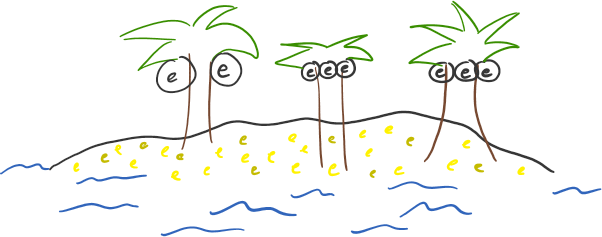
\includegraphics[width=.6\linewidth]{eIsland.png}
\end{center}
\begin{Definition}
  For any $\text{\faScissors}\in \R$, we define:
  \begin{align*}
    e^{\text{\faScissors}}=
    \sum_{\text{\faBicycle}=0}^{\infty} 
    \frac{\text{\faScissors}^{\text{\faBicycle}}}
    {\text{\faBicycle}!}
  \end{align*}
\end{Definition}
This definition sucks, let's try again:
\begin{Definition} We define:
  \begin{align*}
    e=\lim_{\text{\faBicycle}\to\infty}
    \left(1+\frac{1}{\text{\faBicycle}}\right)^{\text{\faBicycle}}
  \end{align*}
  and its side-kick:
  \begin{align*}
    e^{\text{\faScissors}}=\lim_{\text{\faBicycle}\to\infty}
    \left(1+\frac{\text{\faScissors}}
    {\text{\faBicycle}}\right)^{\text{\faBicycle}}
  \end{align*}
\end{Definition}
Shit, we accidentally defined the same thing.
\begin{proof}
  Expand for finite \faBicycle.
\end{proof}
\newpage
\section{Properties of $e$}
\tikz[remember picture,overlay] \node[opacity=0.1,inner sep=0pt] at (current page.center){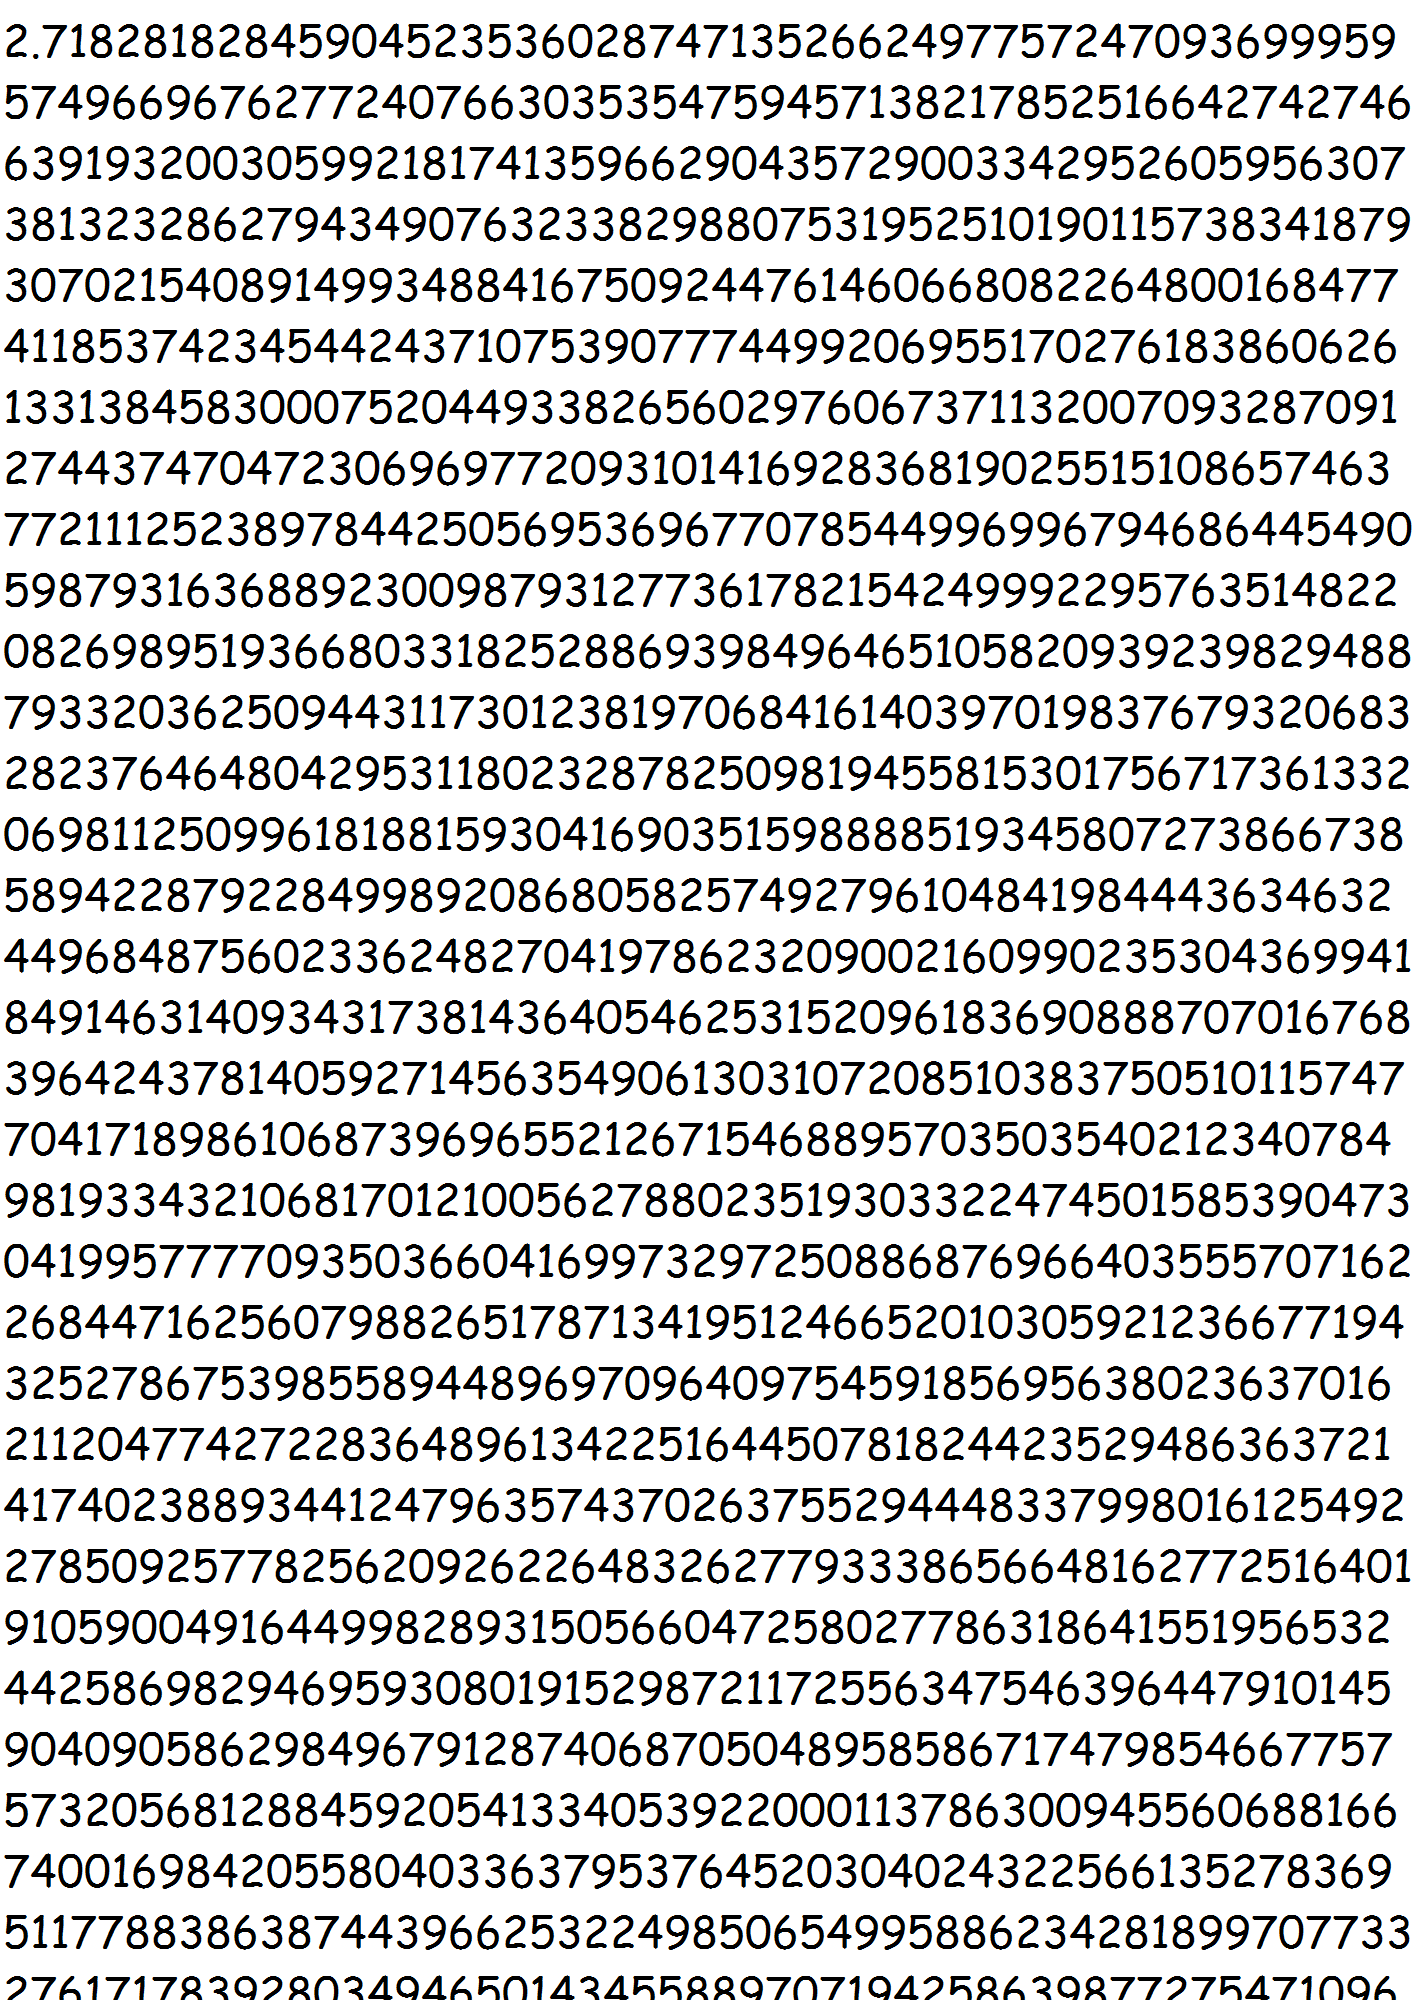
\includegraphics[width=\paperwidth,height=\paperheight]{e_digits.png}};
Ok, so we have this number, but what is it good for? Well, it's a 
good approximation for $2.7$, which is a good approximation for 
$3$, which is a good approximation for $\pi$ for sufficiently bad 
approximations of good. Succinctly:
{\large \begin{align*} e \approx 3\approx\pi \end{align*} }
\begin{Theorem}
  $e$ is irrational
\end{Theorem}
\begin{proof}
  If $e=\frac ab$, then:
  \begin{align*}
    x\coloneq b!\left(\frac{a}{b}-\sum_{n=0}^b \frac{1}{n!}\right)
    =a(b-1)!-\sum_{n=0}^b \frac{b!}{n!}\in \Z
  \end{align*}
  But then by definition of $e=\sum_n\frac{1}{n!}$:
  \begin{align*}
    x = b!\left(\sum_{n=0}^{\infty}\frac{1}{n!}-
    \sum_{n=0}^b \frac{1}{n!}\right)
    =\sum_{n=b+1}^{\infty}\frac{b!}{n!}>0
  \end{align*}
  Next, note that if $n>b$, then $\frac{b!}{n!}<\frac{1}{(b+1)^{n-b}}$, 
  so:
  \begin{align*}
    0<x<\sum_{n=b+1}^{\infty} \frac{1}{(b+1)^{n-b}}
    =\sum_{k=1}^{\infty}\frac{1}{(b+1)^k}=\frac{1}{b}\le  1
  \end{align*}
  so $0<x<1$, a contradiction to $x\in \Z$.
\end{proof}
\newpage
\section{A baker's story}
{\small
A baker wants to bake the perfect cookie: a cookie of $100\%$ chocolate. 
She bakes it, and sets her cookie to cool. In the \faMoonO {}, the 
\queen {} of fairies sends a 
mischevious fairy upon the cookie, to \faBolt {} it with her 
\faMagic $\faMagic^\smallstar\!\smallstar\!\medstar$ 
that turns chocolate into cookie. The next \faSunO, the baker 
finds that her perfect cookie is now $1-1=\text{\faBatteryEmpty}$ 
chocolate! She decides to outsmart the \queen{} by 
splitting her \faBatteryFull{} chocolate cookie 
into two pieces. The \queen {} decides to send two 
fairies to \faBolt \ the halves with their 
\faMagic $\faMagic^\smallstar\!\smallstar\!\medstar$. 
However, being simple creatures of 
$\faMagic^\smallstar\!\smallstar\!\medstar$, neither 
fairy knows which half the other \faBolt{} and each 
\faBolt{} the halves randomly. The next day, the 
baker wakes up to find that her \faBatteryFull{} cookie is now 
$\left(1-\frac{1}{2}\right)^2=\text{\faBatteryQuarter}$ chocolate! She 
decides outsmart the \queen{} by splitting her \faBatteryFull{} 
chocolate cookie into three pieces...}
\begin{center}
  \begin{figure}[ht]
    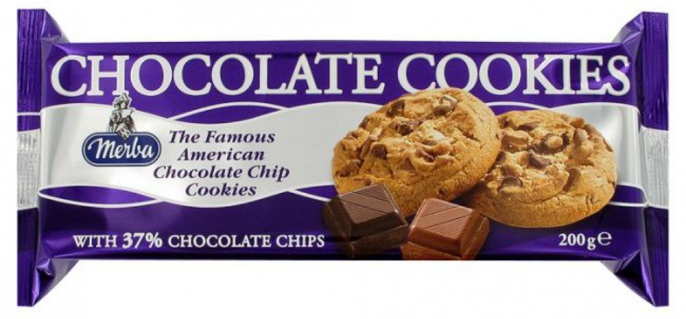
\includegraphics[width=.65\linewidth]{cookies.png}
  \end{figure}
\end{center}
\newpage
\section{The function of the function $e^x$}
Yes, we defined $e^{\text{\faBalanceScale}}$ as a series, or 
as some limit of a sequence, but that's ok. It's still a function, 
with some nice properties.
\begin{enumerate}
  \item $e^x$ is a monotonically increasing positive function 
    from $\R$ to $\R$.
  \item $e^{x+y} = e^x e^y$, $e^0=1$ (homomorphism!)
  \item If you made a slide in the shape of the plot of $y=e^x$, 
    you will never stop slidin' leftward.
\end{enumerate}
\begin{center}
  \begin{tikzpicture}[scale=.5]
    \draw[->] (-5,0) -- (2,0) node[right] {$x$};
    \draw[->] (0,-2) -- (0,6) node[above] {$y$};
    \draw[<->,domain=-5:2,smooth,variable=\x,red,thick] 
    plot ({\x},{exp(\x)});
    \node [scale=.5,below right] at (0,0) {$0$};
    \node [scale=.5,below] at (-1,0) {$-1$};
    \node [scale=.5,below] at (-2,0) {$-2$};
    \node [scale=.5,below] at (-3,0) {$-3$};
    \node [scale=.5,below] at (-4,0) {$-4$};
    \node [scale=.5,below] at (1,0) {$1$};
    \node [scale=.5,below] at (2,0) {$2$};
    \node [scale=.5,left] at  (0,-1) {$-1$};
    \node [scale=.5,left] at  (0,1) {$1$};
    \node [scale=.5,left] at  (0,2) {$2$};
    \node [scale=.5,left] at  (0,3) {$3$};
    \node [scale=.5,left] at  (0,4) {$4$};
    \node [scale=.5,left] at  (0,5) {$5$};
    \node [scale=.5,below right] at (0,0) {$0$};
    \node [scale=.7,above,red,very thick] at (-5,0) {$\exp(x)=e^x$};
  \end{tikzpicture}
\end{center}
But most importantly:
\begin{Theorem}
  $\frac{d}{dx} e^x = e^x$($\Rightarrow \frac{d}{dx}e^{cx}=ce^{cx}$ by 
  \faChain \ rule).
\end{Theorem}
\begin{proof}
  Use the first definition, and differentiate term by term.
\end{proof}
\newpage
\begin{quote}
  \enquote{$\log(x)$, being the inverse function of $e^x$, has always been 
  controversial. Some say that $\log$ makes them feel $\text{\faEye}^
  \text{\faFeed}_{\text{\faMusic}_{\text{\faOpenid}}}\text{\faHandLizardO}$
  \mute{Cat and mouse, oil and water, Israel 
  and Palestine. None compare to the battle between $e$ and $\log$.}}
\end{quote}
\section*{Captain's log day 1: $e$-log-ical musings}
\begin{verbatim}
>How does a number theorist drown?
>loglogloglog
>What do you get when you integrate 
 one over cabin with respect to cabin?
>log cabin
>No, it's a houseboat, you forgot to 
 add the c!
>No, it's a priceless yacht, you 
 disregarded the absolute value
\end{verbatim}
\setcounter{section}{6}
\begin{center}
  \begin{figure}[ht]
    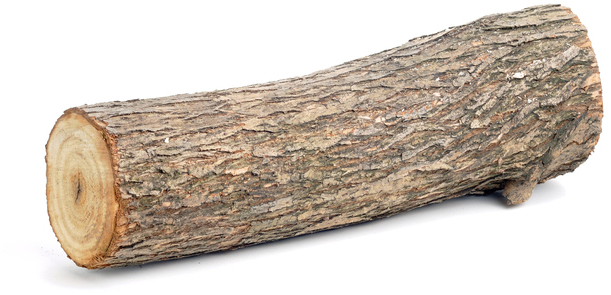
\includegraphics[width=.57\linewidth]{log.png}
    \caption{log for scale. Scale pictured on previous page}
  \end{figure}
\end{center}
\newpage
\section{$e$ is \faCutlery \ for more than $\R$}
\tikz[remember picture,overlay] \node[opacity=0.6,inner sep=0pt] at (current page.center){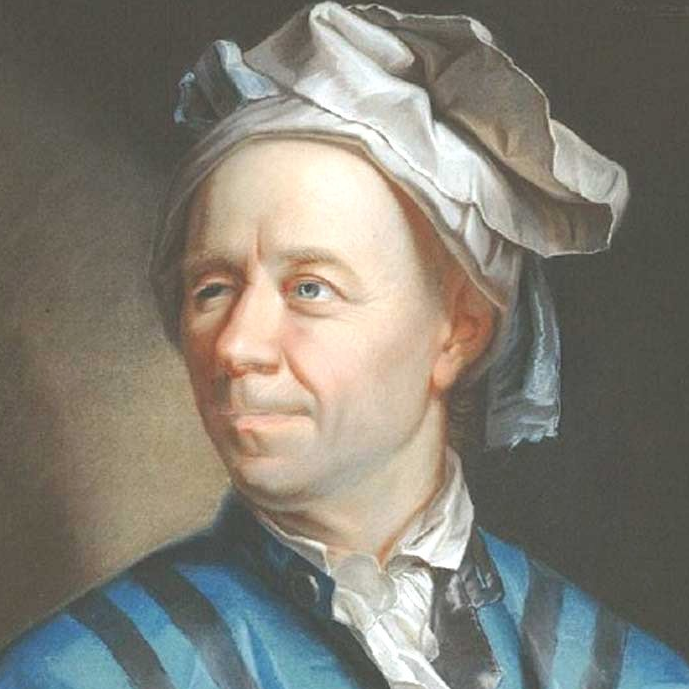
\includegraphics[width=\paperwidth,height=\paperheight]{Euler.png}};
\mute{The expression $e^x =\sum_n \frac{x^n}{n!}$ makes sense when 
$x$ is a real number. However, we can generalize. In order for 
that expression to make sense, all we really need is:
\begin{center}
  \begin{figure}[ht]
    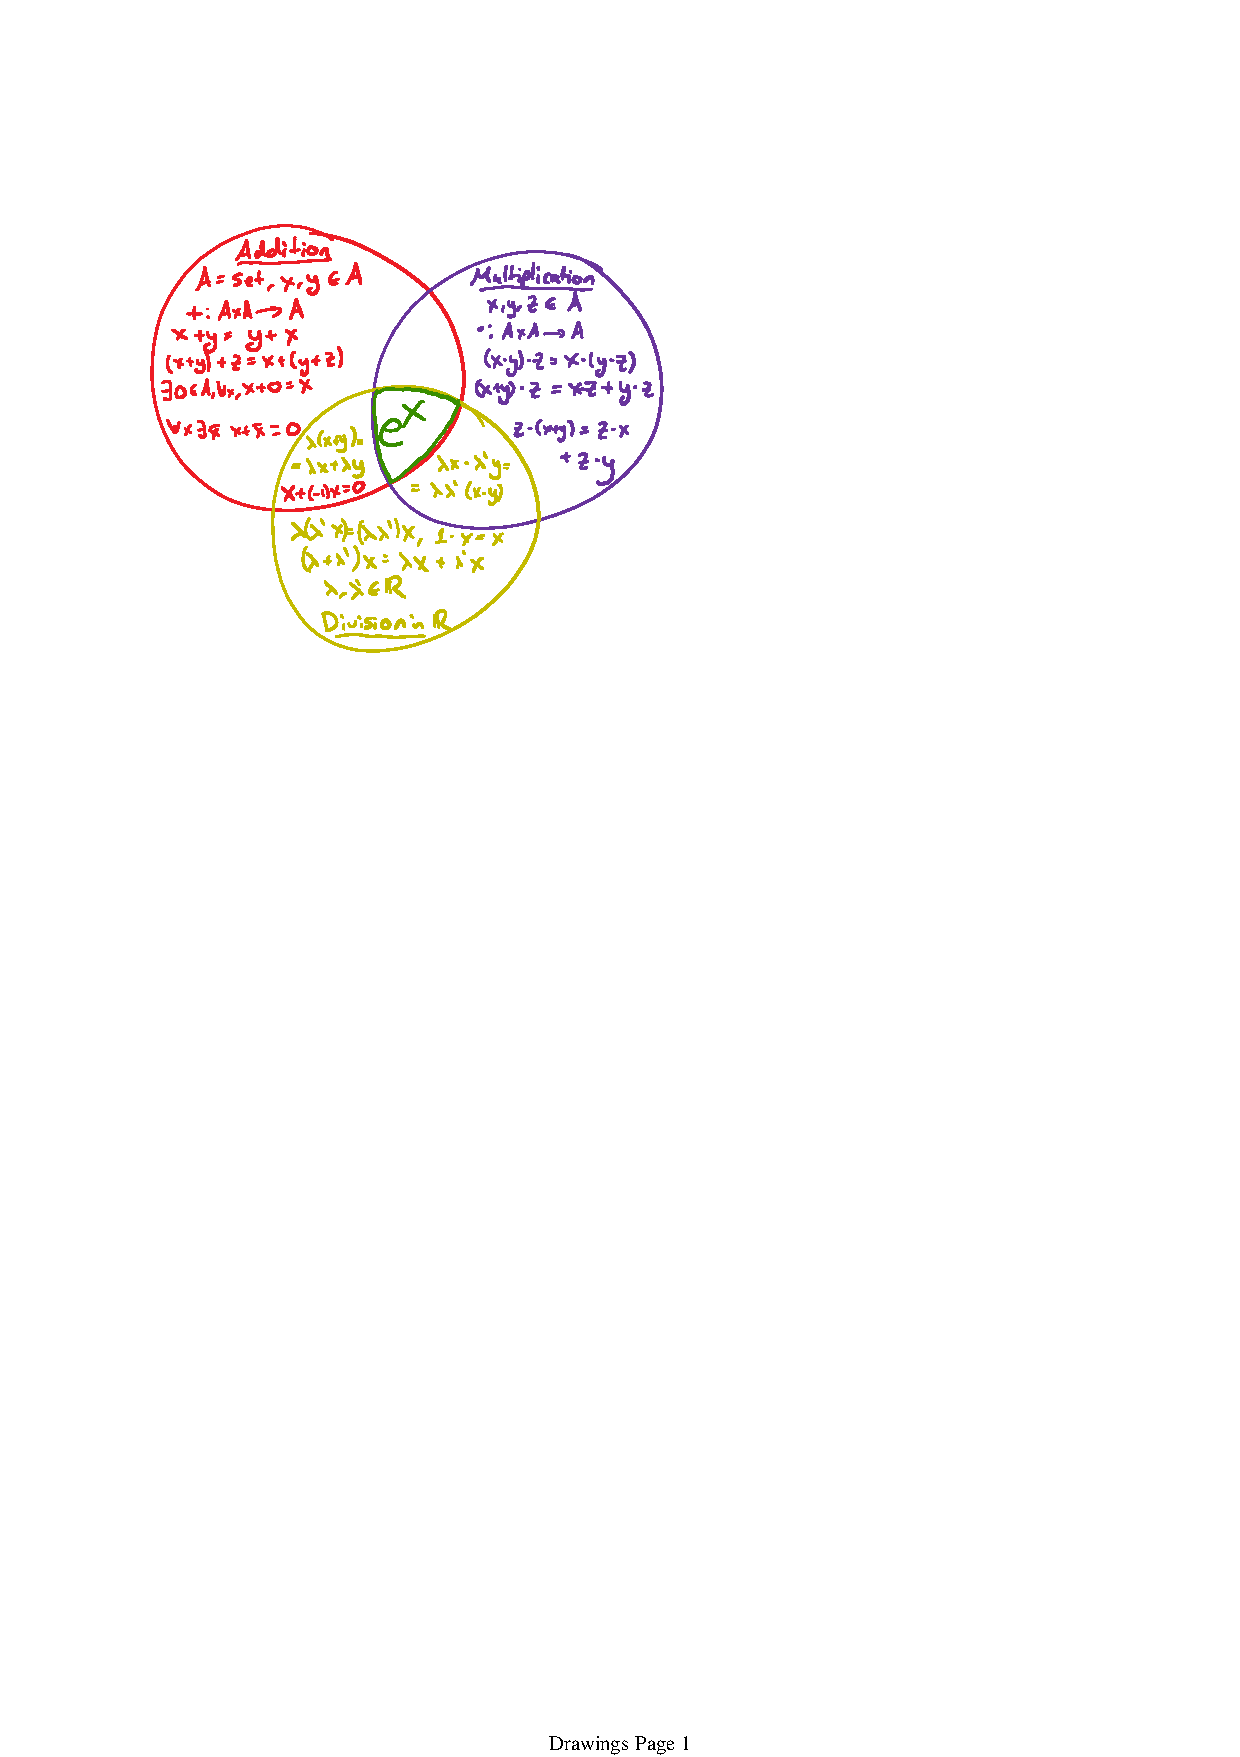
\includegraphics[trim={2.5cm 18.7cm 9.7cm 3.8cm},clip, width=.7\linewidth]{AlgebraVenn_Whole.pdf}
  \end{figure}
\end{center}
This structure is called a {\bf REAL ALGEBRA}.}

Nothing\footnote{well, some things, like being able to take powers, sums, 
division over $\Q$, convergence...} 
prevents $x$ from being another kind of number. 
Another number? Different numbers? Other numbers? Complex numbers.
%If $z=a+bi$, we define $e^z=\sum_n\frac{1}{n}z^n}$. 
%IDEA: Euler picture background fade in
\begin{Theorem}
  Let $a+bi=z\in \C$. Then
  \begin{align*}
    e^z = e^ae^{bi}=e^a(\cos(b)+i\sin(b))
  \end{align*}
\end{Theorem}
\begin{proof}
  To prove $e^z=e^ae^{bi}$, we have to use multinomial theorem 
  on the first definition, like in the real case. To 
  prove $e^{bi}=\cos(b)+i\sin(b)$, exponentiate and 
  and use Taylor's formulas for $\sin$ and $\cos$.
\end{proof}
%IDEA: for the bottom here, have the matrix code background fade in to cover the example.
\begin{Example}
  We can take the exponent of a square matrix to get another 
  matrix. \\
  It turns out that if $A\in \text{Mat}(n)$, then $e^Ae^{-A} = I_n$, so 
  $e^A$ is always invertible. 
\end{Example}
However, some of the exponent rules don't work. If
$A = \left(\begin{smallmatrix}0&1\\0&0\end{smallmatrix}\right)$ 
and $B =\left(\begin{smallmatrix}0&0\\1&0\end{smallmatrix}\right)$, 
then:
\begin{align*}
 e^Ae^B\neq e^B e^A
 \end{align*}
\newpage
\section{$e^x$-tra-ordinary differential equations}
\begin{Example}
  Consider the {\bf system} of linear differential 
  equations\footnote{Whoa what's this? We only learned what $e$ 
  was a few pages ago and now we're doing differential equations?}:
  \begin{align*}
    f_1'&=a_{1,1}f_1+\cdots+a_{1,n}f_n\\
    f_2'&=a_{2,1}f_1+\cdots+a_{2,n}f_n\\
    \vdots&\qquad \vdots\qquad \ \ddots\qquad  \vdots\\
    f_n'&=a_{n,1}f_1+\cdots+a_{n,n}f_n
  \end{align*}
  AKA $\frac{d}{dx}\vec f = A \vec f$, 
  where ${A=(a_{ij})_{ij}}$ is a matrix of constants and 
  $\vec f = (f_1,\ldots,f_n)$ is a vector of functions of a 
  single variable. \\
  Let $\vec f(0)=v\in \R^n$ be the initial condition. Then:
  \begin{align*}
    \frac{d}{dx} e^{Ax}v=\left(\frac{d}{dx} e^{Ax}\right)v
    +e^{Ax}\frac{d}{dx}v = Ae^{Ax}v
  \end{align*}
  Meaning that $\vec f = e^{Ax}v$ solves the system, and meets the 
  initial condition $\vec f(0) = e^{0}v = I_nv=v$.
\end{Example}
\begin{Remark}
  This also works when replacing a matrix with any linear 
  operator. This is how physicists solve 
  Schr\includegraphics[width=10pt]{cat.png}dinger's equation.
\end{Remark}
\end{document}
